\section{Conception des données}
Pour structurer notre base de données relationnelle sous PostgreSQL, nous avons élaboré un Diagramme de Classes UML détaillé. Afin d'assurer une évolutivité maximale et de faciliter la maintenance, nous avons adopté une approche de conception modulaire orientée domaine (Architecture par domaine). Cela permet d'isoler logiquement les différentes responsabilités de l'application SmartFit. 

Voici la présentation détaillée de chaque domaine métier constituant notre système :

\subsection{1. Gestion des Utilisateurs et Authentification}
\textbf{Description} : Ce module constitue le cœur sécurisé du système. Il gère la création, l'authentification et l'autorisation des différents acteurs de la plateforme (Sportifs, Coachs, Administrateurs). Il centralise les données personnelles, les métriques de base (poids, taille, niveau) et assure la sécurité des sessions via un système de jetons (tokens).
\begin{figure}[H]
    \centering
    
\includegraphics[width=\textwidth,height=12cm,keepaspectratio]{img/diagramme-classe/1.png}
    \caption{Modèle de données : Gestion des Utilisateurs}
\end{figure}

\subsection{2. Gestion de la Relation Coach-Sportif}
\textbf{Description} : Ce domaine encadre les interactions professionnelles et commerciales entre les utilisateurs. Il permet de gérer le cycle de vie complet d'une demande d'accompagnement (envoi, acceptation, refus) et conserve un historique détaillé des négociations (propositions tarifaires, commentaires), assurant ainsi une mise en relation transparente et tracée.
\begin{figure}[H]
    \centering
    
\includegraphics[width=\textwidth,height=12cm,keepaspectratio]{img/diagramme-classe/2.png}
    \caption{Modèle de données : Relation Coach-Sportif}
\end{figure}

\subsection{3. Conception et Planification des Programmes}
\textbf{Description} : Dédié à la structuration du parcours d'entraînement, ce module permet aux coachs de concevoir des programmes sportifs complets. Il offre aux sportifs la possibilité de formuler des demandes personnalisées, de s'inscrire à des programmes existants et d'organiser leurs séances d'entraînement selon un mode de planification manuel ou automatisé.
\begin{figure}[H]
    \centering
    
\includegraphics[width=\textwidth,height=12cm,keepaspectratio]{img/diagramme-classe/3.png}
    \caption{Modèle de données : Planification des Programmes}
\end{figure}

\subsection{4. Journalisation et Suivi des Activités}
\textbf{Description} : Ce domaine est responsable de la traçabilité de l'effort physique. Il enregistre l'exécution concrète des séances (cardio, musculation), détaille chaque exercice réalisé (répétitions, charges, distance) et évalue le statut de complétion. Cela permet de constituer un journal de bord précis des performances réelles de l'utilisateur.
\begin{figure}[H]
    \centering
    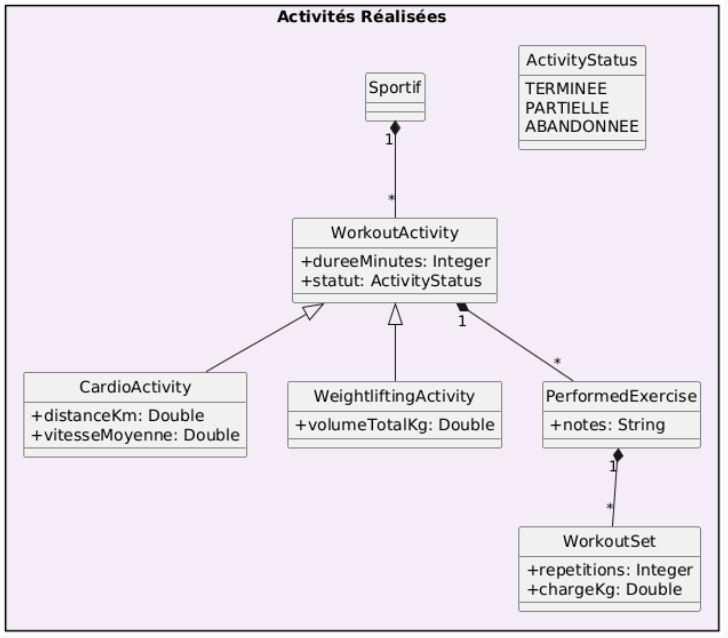
\includegraphics[width=\textwidth,height=12cm,keepaspectratio]{img/diagramme-classe/4.png}
    \caption{Modèle de données : Journalisation et Activités}
\end{figure}

\subsection{5. Référentiel et Catalogue d'Exercices}
\textbf{Description} : Il s'agit de la bibliothèque centralisée de l'application. Ce module répertorie tous les mouvements et exercices disponibles, classés par catégorie (cardio, musculation, stretching) et par niveau de difficulté. Il intègre également des ressources pédagogiques (vidéos, consignes d'exécution) pour garantir une pratique sportive correcte et sécurisée.
\begin{figure}[H]
    \centering
    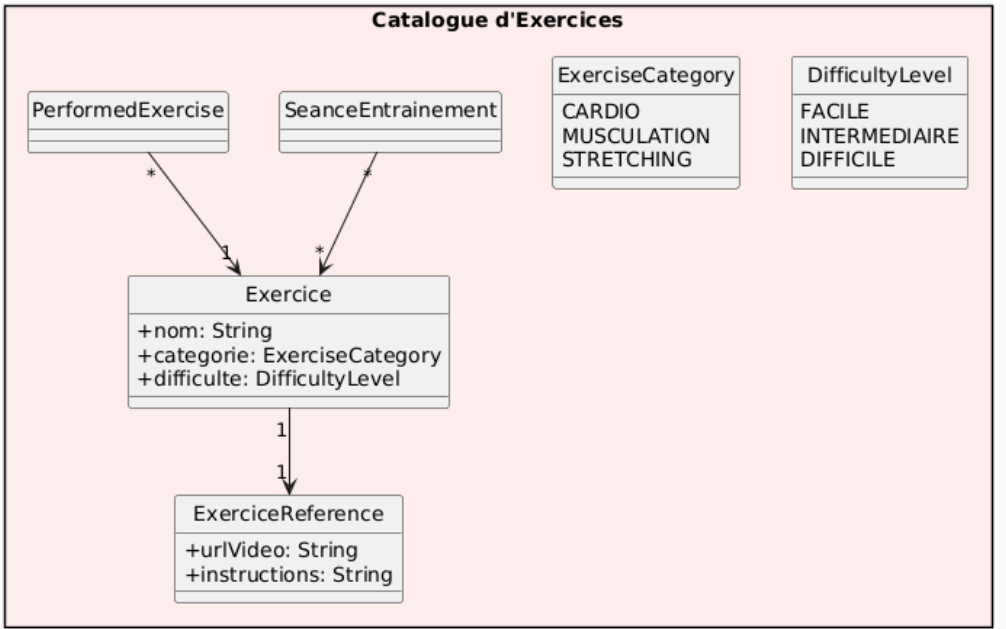
\includegraphics[width=\textwidth,height=12cm,keepaspectratio]{img/diagramme-classe/5.png}
    \caption{Modèle de données : Catalogue d'Exercices}
\end{figure}

\subsection{6. Gestion de la Santé et de la Nutrition}
\textbf{Description} : Ce domaine complète l'approche sportive par un suivi diététique structuré. Il permet de définir des plans nutritionnels adaptés aux régimes spécifiques de chaque utilisateur (omnivore, végétarien, keto, etc.). Il gère la répartition des repas, le contenu des assiettes et le suivi des objectifs caloriques quotidiens.
\begin{figure}[H]
    \centering
    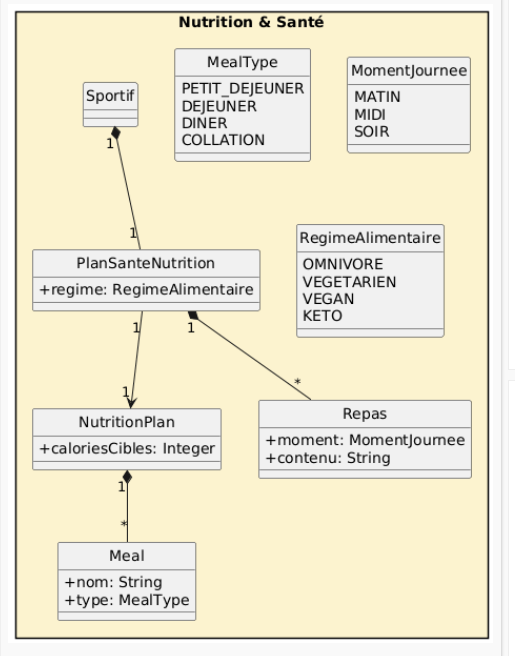
\includegraphics[width=\textwidth,height=12cm,keepaspectratio]{img/diagramme-classe/6.png}
    \caption{Modèle de données : Santé et Nutrition}
\end{figure}

\subsection{7. Analytique, Suivi et Intelligence Artificielle}
\textbf{Description} : Centré sur l'évaluation de la progression, ce module agrège les métriques de bien-être quotidien (sommeil, humeur, poids) et les statistiques hebdomadaires (calories brûlées). Il intègre également des fonctionnalités avancées basées sur l'Intelligence Artificielle, telles que l'analyse posturale par vision par ordinateur (Computer Vision), offrant un retour d'expérience hautement qualitatif.
\begin{figure}[H]
    \centering
    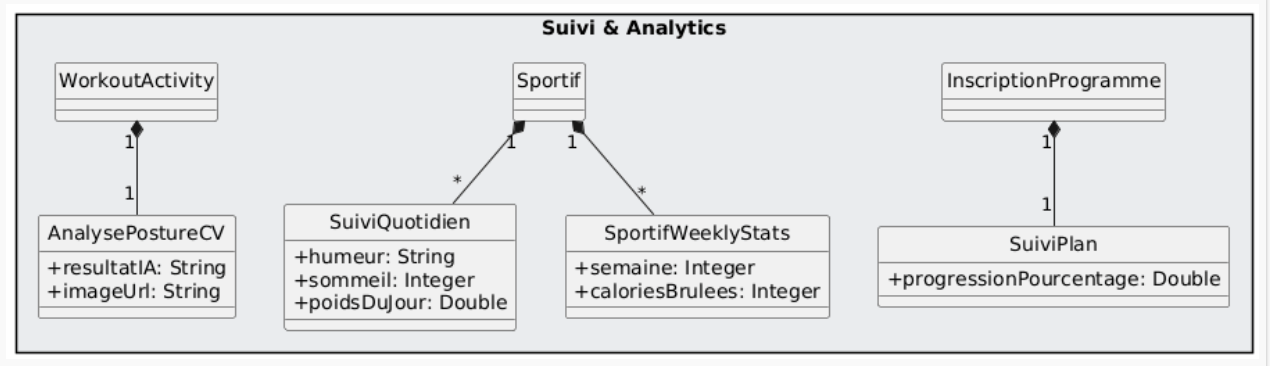
\includegraphics[width=\textwidth,height=12cm,keepaspectratio]{img/diagramme-classe/7.png}
    \caption{Modèle de données : Analytique et Intelligence Artificielle}
\end{figure}

\subsection{8. Espace Social et Communication}
\textbf{Description} : Ce module favorise l'engagement et la rétention en apportant une dimension communautaire à la plateforme. Il orchestre les échanges via une messagerie interne, gère le système de notifications (rappels, alertes) et permet aux utilisateurs d'interagir publiquement à travers des publications et des commentaires.
\begin{figure}[H]
    \centering
    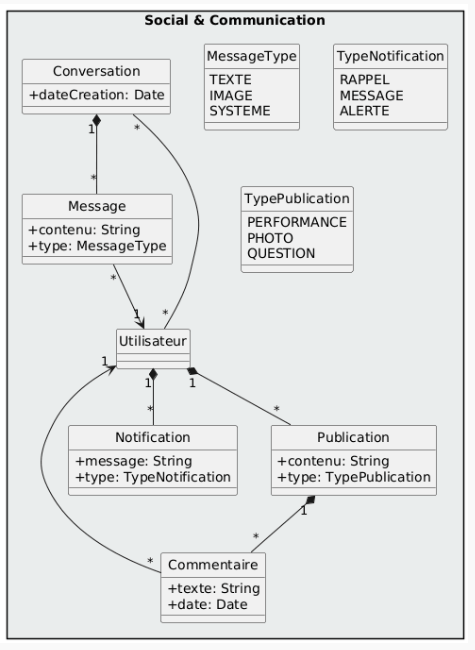
\includegraphics[width=\textwidth,height=12cm,keepaspectratio]{img/diagramme-classe/8.png}
    \caption{Modèle de données : Espace Social et Communication}
\end{figure}

\subsection{9. Équipements, Abonnements et Gamification}
\textbf{Description} : Ce domaine transversal gère l'environnement matériel et ludique du sportif. Il prend en charge la gestion des différents paliers d'abonnement (Gratuit, Premium, VIP), l'intégration d'appareils connectés (IoT), l'association à des salles de sport physiques, ainsi que les éléments de motivation comme les défis et la création de groupes d'entraînement.
\begin{figure}[H]
    \centering
    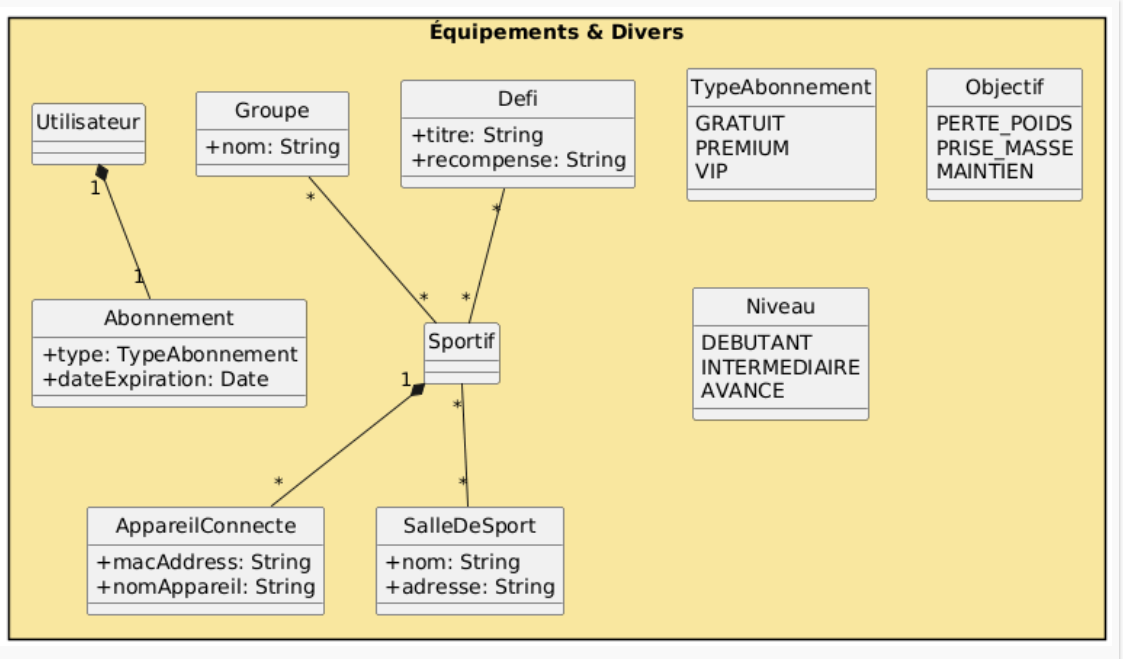
\includegraphics[width=\textwidth,height=12cm,keepaspectratio]{img/diagramme-classe/9.png}
    \caption{Modèle de données : Gamification et Abonnements}
\end{figure}
